\documentclass[11pt]{article}
\usepackage[a4paper,landscape,margin=0.72in]{geometry}
\usepackage[T1]{fontenc}
\usepackage{lmodern,amsmath,amssymb,graphicx,hyperref}
\title{Rational-point Jacobian condition and the actual point-stalk DVR}
\author{Formal proof packet}
\date{28 October 2026}
\begin{document}
\maketitle
\noindent This packet records a checked pointwise differential equivalence and conditional DVR results for the actual weighted-$\operatorname{Proj}$ point stalk. It contains no target result, experiment, or cost ratio. The Lean source, direct compiler log, SVG graph, and CSV status table accompany this PDF.

\section*{Checked boundary}
Let $K$ be any field, $f(X)=X^5+a_3X^3+a_2X^2+a_1X+a_0$, and $(a,y)$ a rational point of $y^2=f(a)$. The checked derivative lemma identifies the explicit $f'(a)$ used by the local-parameter proof with the formal derivative of the actual quintic. The checked equivalence is
\[
(2y\ne0\;\lor\;f'(a)\ne0)\quad\Longleftrightarrow\quad
(\partial_y(y^2-f(x))|_{(a,y)}\ne0\;\lor\;\partial_x(y^2-f(x))|_{(a,y)}\ne0).
\]
This is an algebraic equivalence between the source's explicit partial derivatives. It has no characteristic restriction. Under separability of $f$, either nonzero partial gives a DVR for the affine rational-point localization and the actual weighted-$\operatorname{Proj}$ point stalk. The two local parameters are $x-a$ in the first case and $y-y_0$ in the second. The projective theorem also accepts the nonzero-partial premise directly.

\section*{Verification and scope}
Direct pinned Lean 4.34.1 compilation exited zero against Mathlib revision \texttt{d13f23b723b8a846827a245b89c10fc7d3f11612}. Five printed axiom audits list only \texttt{propext}, \texttt{Classical.choice}, and \texttt{Quot.sound}; no \texttt{sorryAx}. Source SHA-256:
\par\noindent{\small\texttt{b662ea86f06b6ff9066d283272304f83df49aee3a3d8fdaad19a4740f471c283}}.\par
The source combines the checked \texttt{WeightedProjNonbranchDVR} and \texttt{WeightedProjDerivativePointDVR} theorems. An equivalence with a scheme-theoretic \texttt{Smooth} predicate, global principal-divisor/$\mathrm{Pic}^0$ transport, and compiled Rust semantics remain open. This result makes no order-allocation assertion in characteristic two.

\clearpage
\section*{Proof dependencies and open gates}
\begin{center}
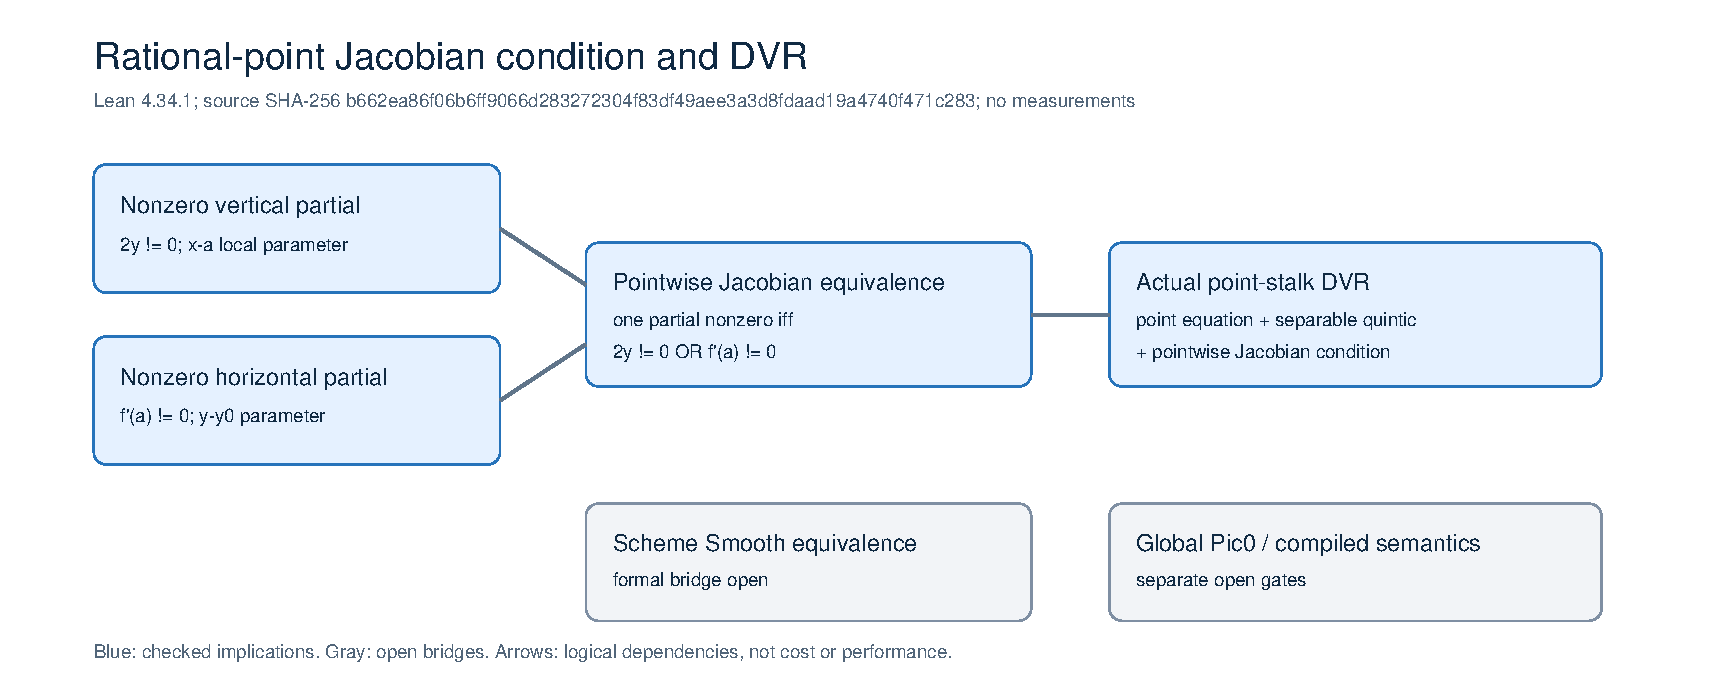
\includegraphics[width=0.96\textwidth,height=0.76\textheight,keepaspectratio]{smooth-point-dvr-figure.pdf}
\end{center}
\noindent Blue nodes are checked implications. Gray nodes remain open. Arrows show proof dependencies, not measured performance.
\end{document}
